\section{Topologisk sortering}
Topologisk sortering er en ordning av noder i en DAG slik at dersom det finnes en vei fra $ v_i $ til $ v_j $ i grafen kommer $ v_i $ før $ v_j $ i sorteringa. En topologisk sortering er ikke nødvendigvis entydig bestemt, ofte finnes det veldig mange. Hvis en graf er syklisk eksisterer det ikke en topologisk sortering av grafen. Vi ser på et eksempel: \index{topologisk sortering}

\begin{example} Gitt følgende graf, finn alle topologiske sorteringer.
\begin{figure}[h!]
\centering
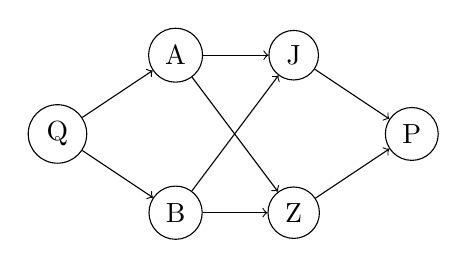
\begin{tikzpicture}[->]
\tikzstyle{v} = [circle, draw=black]
\tikzstyle{e} = [draw=black]

\node[v] (Q) at (-3, 0) {Q};
\node[v] (A) at (-1.5, 1) {A};
\node[v] (B) at (-1.5, -1) {B};
\node[v] (J) at (0, 1) {J};
\node[v] (Z) at (0, -1) {Z};
\node[v] (P) at (1.5, 0) {P};

\draw[e] (Q) to (A);
\draw[e] (Q) to (B);
\draw[e] (A) to (J);
\draw[e] (B) to (Z);
\draw[e] (B) to (J);
\draw[e] (A) to (Z);
\draw[e] (J) to (P);
\draw[e] (Z) to (P);
\end{tikzpicture}
\end{figure}

Vi ser at Q har inngrad 0, det er derfor et logisk sted å begynne. Etter Q kommer A og B. Vi ser at vi kan ikke gå videre fra A før uten å ha vært innom B, siden både J og Z er avhengige av B. Tilsvarende kan vi ikke gå videre fra B før vi har vært innom A. Til slutt ser vi at P er avhengig av både J og Z. Begge de to må derfor komme før P i sorteringa. Vi har da dekt alle mulige utfall. Vi kan liste opp alle mulige sorteringer:
\begin{itemize}
\item Q, A, B, J, Z, P
\item Q, B, A, J, Z, P
\item Q, A, B, Z, J, P
\item Q, B, A, Z, J, P
\end{itemize}

Vi kan ta med et moteksempel også: Q, A, J, B, Z, P er ikke en gyldig topologisk sortering siden J kommer før B i sorteringa, men i grafen ser vi at J er avhengig av B (det går en kant fra B til J).
\end{example}